One of the defining properties of topological insulators is the presence of conducting edge states with an insulating bulk. The example considered here in sec. \ref{sec:ti_exemples} is a two dimensionnal material and its edge is therefore one-dimensionnal. The QH and QSH effects both involve one-dimensionnal conduction. In one dimension, electrons can only either move forward of backward on the edge of the sample and this restriction is central for Hall effects. \cite{qi_quantum_2010}. 
\subsection{QH}
The QH effect occurs in two dimensionnal semiconductor electron gas with a strong applied magnetic field \cite{qi_quantum_2010}. It is robust to the addition of impurities in a topological way because the conducting edge states only carry current in one direction on a given side of the sample. Adding an impurity can't lead to backscattering of the electrons because there are simply no backward moving states they can scatter into \cite{qi_quantum_2010}. 

\begin{figure}[h]
    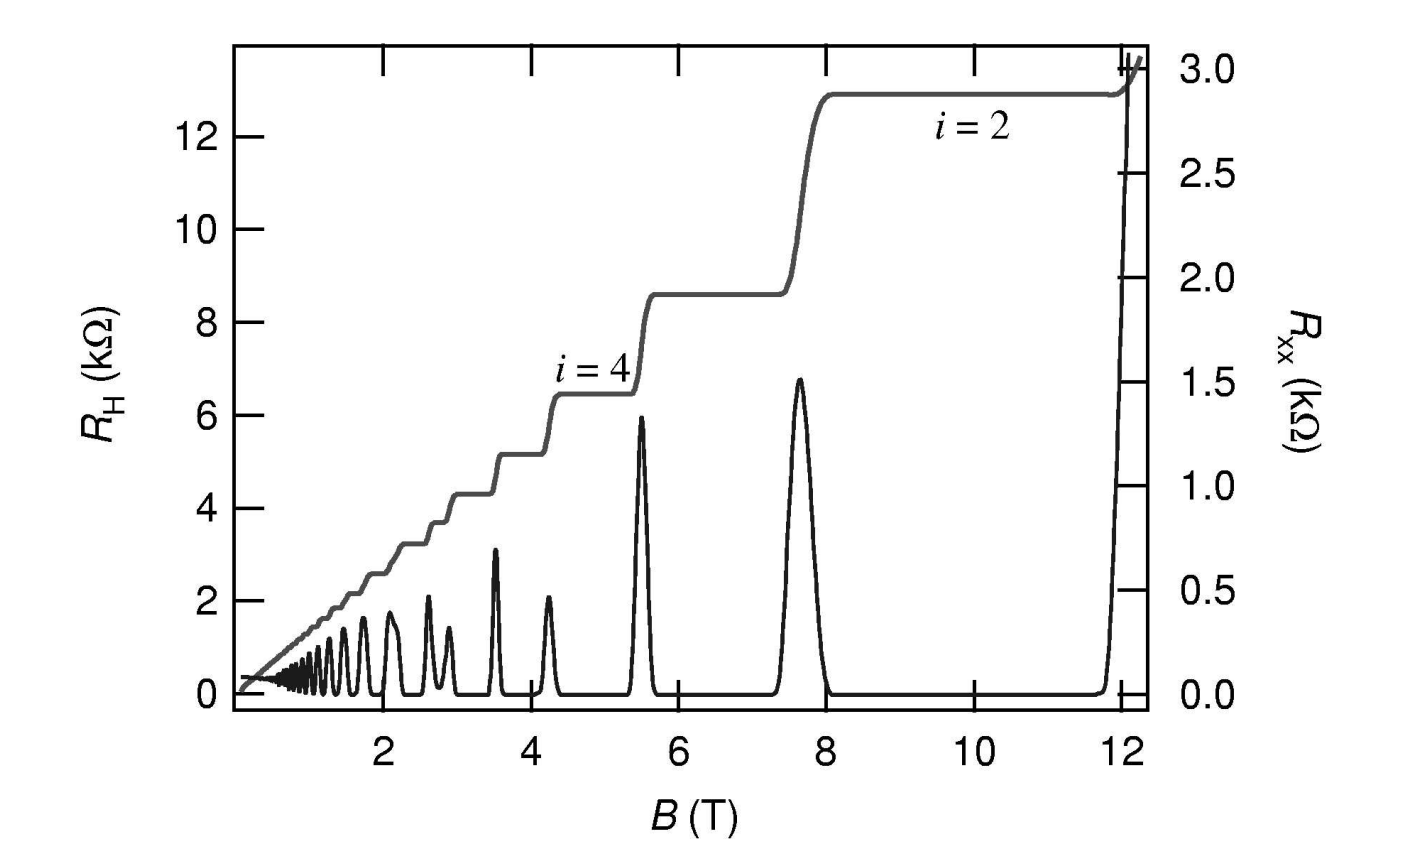
\includegraphics[width=\columnwidth]{sections/visuel/Hall_effect.png}
    \caption{Hall Effect mersurments. The upper curve represent the Hall resistance ($R_h \propto \frac{1}{\sigma_{xy}}$) and shows its plateaus while the lower one represent $R_{xx} \propto \rho_{xx}$ and shows its vanishing. Both curve are a function of the magnetic feild. \cite{jeckelmann_quantum_nodate}}
    \label{fig:Hall_effet}
\end{figure}

The QH effect consists of a two simultanious and related phenomena. The quantized \textit{Hall conductivity} $\sigma_{xy}(=\frac{I_x}{V_y})$ and the vanishing of the $\rho_{xx}$ resistivity in a 2D electron gas. The link with topology is fairly direct since the Hall Conductivity is directly proportional to the Chern number! In fact we have.
\begin{equation}
\sigma_{xy} = \mathcal{C}\frac{e^2}{\hbar}
\end{equation}

where $\mathcal{C}$ is the Chern number.

\begin{figure}[h!]
    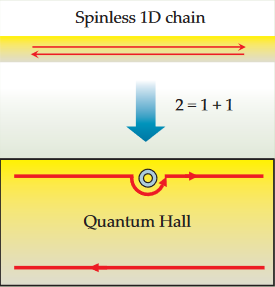
\includegraphics[scale = 0.7]{sections/visuel/spinless.png}
    \caption{Schematic representation of the conduction chanels in a spinless quantum Hall system.\cite{qi_quantum_2010}}
    \label{spinless}
\end{figure}



\subsubsection{Chern number}

% The Chern number is a topological invariant closely related to the Euler characteristic. In fact you can write the \textit{topological solid} equivalent of the \textit{Gauss-bonnet} theorem 



\subsubsection{Impossiblity of backscattering}

\subsubsection{In which material does it happen}


\subsection{QSH}

\begin{figure}[h!]
    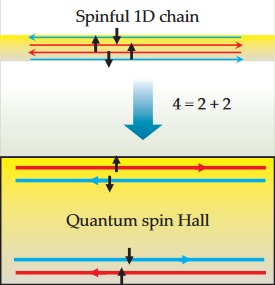
\includegraphics[scale = 0.7]{sections/visuel/spinful.png}
    \caption{Schematic representation of the conduction chanels in a spinlful quantum Hall system.}
    \label{spinful}
\end{figure}

% Talk about the fact that the states are topologicaly protected since their edge states survive the addition of impurities \cite{kane_this_2011}